\section[ЛР №4. Модель обслуживания IaaS, OpenStack]{Лабораторная работа №4. \\
Модель обслуживания IaaS на примере создания инстанса в OpenStack}

\textbf{Цель работы:} ознакомиться с веб-интерфейсом OpenStack, научиться настраивать сеть, создавать инстансы и управлять ими в OpenStack, ознакомиться с преимуществами использования IaaS-решений по сравнению с PaaS.

\subsection{Краткие сведения об OpenStack}

Ранее в лабораторной работе №3, уже использовалось готовое PaaS-решение от облачного провайдера Heroku.
Однако если же нужно использовать более гибкие IaaS-решения или же есть желание самому стать облачным провайдером, то необходимо использование инструментов, таких как OpenStack.

С помощью OpenStack можно создавать платформы облачных вычислений для частных и публичных облаков.
OpenStack был начат как совместный проект между Rackspace и NASA в 2010 году.
С 2012 года им управляет некоммерческая организация OpenStack Foundation.

Теперь OpenStack поддерживают более чем 500 сторонних организаций.
OpenStack является открытым проектом, исходные коды распространяются под лицензией Apache 2.0.

Помимо обеспечения IaaS-решений, OpenStack развивалась с течением времени, чтобы предоставлять другие услуги, как базы данных, системы хранения данных и прочее.

Благодаря модульной архитектуре OpenStack, любой желающий может добавить дополнительные компоненты, чтобы получить специфические особенности или функциональные возможности.

Некоторые из основных компонентов OpenStack:
\begin{itemize}
    \item Keystone, инструментом идентификации пользователей;
    \item Nova, диспетчер облачного процесса вычислений;
    \item Horizon, панель управления для OpenStack;
    \item Neutron, реализация сети в качестве сервиса, обеспечение сетевых возможностей для различных компонентов;
    \item Glance, используется для управления образами ОС, которые требуются для работающих экземпляров (инстансов);
    \item Swift, распределенное хранилище высокой доступности;
    \item Cinder, блочное хранилище;
    \item Heat, инструмент оркестровки, позволяет запускать готовые облачные архитектуры из шаблонов, описанных текстом;
    \item Celiometer, инструмент для сбора различных статистических данных в облаке.
\end{itemize}

Каждый из компонентов OpenStack является также модульным.

Например, с помощью Nova можно выбрать гипервизор в зависимости от требований, libvirt (QEMU/KVM), Hyper-V, VMWare, XenServer, Xen с libvirt.

\clearpage

\begin{figure}[ht]
    \centering
    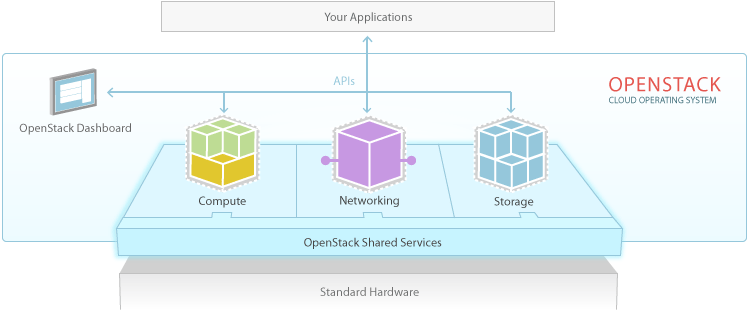
\includegraphics[width=\linewidth]{openstack}
    \caption{Общая схема OpenStack}\label{pic:openstack}
\end{figure}

Преимущества использования OpenStack:
\begin{itemize}
    \item решение с открытым исходным кодом;
    \item платформа облачных вычислений для публичных и частных облаков;
    \item предлагает гибкое и настраиваемое окружение;
    \item обеспечивает высокий уровень безопасности;
    \item облегчает автоматизацию на протяжении всех этапов жизненного цикла облака;
    \item за счет снижения затрат на управление системой и отсутствия привязанности к вендору, это может быть экономически эффективным.
\end{itemize}

\subsection{Порядок выполнения работы}

Для выполнения данной лабораторной работы необходим аккаунт на Facebook.

Пример работы с TryStack представлен в прил.~\ref{pril:f}.

\begin{enumerate}
    \item Вступить в группу TryStack на Facebook;
    \item Авторизоваться на сервисе TryStack и ознакомиться с интерфейсом OpenStack;
    \item Согласно прил.~\ref{pril:f} настроить окружение для создания инстанса;
    \item Создать тестовый инстанс и разместить любое приложение (по желанию);
    \item Проверить работоспособность приложения в облаке.
\end{enumerate}

\subsection{Контрольные вопросы}
\begin{enumerate}
    \item В чем преимущество и недостатки использования IaaS перед PaaS?
    \item Назовите несколько примеров облачных поставщиков IaaS?
    \item Почему использование SSH-ключей безопаснее чем парольная аутентификация?
\end{enumerate}

\clearpage
